\documentclass{article}

\usepackage[version=3]{mhchem} % Package for chemical equation typesetting
\usepackage{siunitx} % Provides the \SI{}{} and \si{} command for typesetting SI units
\usepackage{graphicx} % Required for the inclusion of images
\usepackage{natbib} % Required to change bibliography style to APA
\usepackage{amsmath} % Required for some math elements 
\usepackage{float}
\setlength\parindent{0pt} % Removes all indentation from paragraphs

\renewcommand{\labelenumi}{\alph{enumi}.} % Make numbering in the enumerate environment by letter rather than number (e.g. section 6)

%\usepackage{times} % Uncomment to use the Times New Roman font

%----------------------------------------------------------------------------------------
% DOCUMENT INFORMATION
%----------------------------------------------------------------------------------------

\title{Exploring Weather Trends \\ Data Analyst Nanodegree Program} % Title

\author{MingCong (Luca) \textsc{Zhou}} % Author name

\date{\today} % Date for the report

\begin{document}

\maketitle % Insert the title, author and date

% If you wish to include an abstract, uncomment the lines below
% \begin{abstract}
% Abstract text
% \end{abstract}

%----------------------------------------------------------------------------------------
% SECTION 1
%----------------------------------------------------------------------------------------

\section{Objective}
In this project, we analyze local and global temperature data and compare the temperature trends in my city to overall global temperature trends.

% If you have more than one objective, uncomment the below:
% \begin{description}
% \item[First Objective] \hfill \\
% Objective 1 text
% \item[Second Objective] \hfill \\
% Objective 2 text
% \end{description}
 
%----------------------------------------------------------------------------------------
% SECTION 2
%----------------------------------------------------------------------------------------

\section{Extract the data}
Our goal is to extract both the world averages and my city’s averages. To find out what cities the database offering for Canada, we can use the following SQL query:
\begin{center} SELECT city FROM city\_list WHERE country = 'Canada'; \end{center}

After the data is retrieved from the database, as we can see in Figure 1, London is the closest big city from the result. 
\begin{figure}[H]
  \begin{center}
    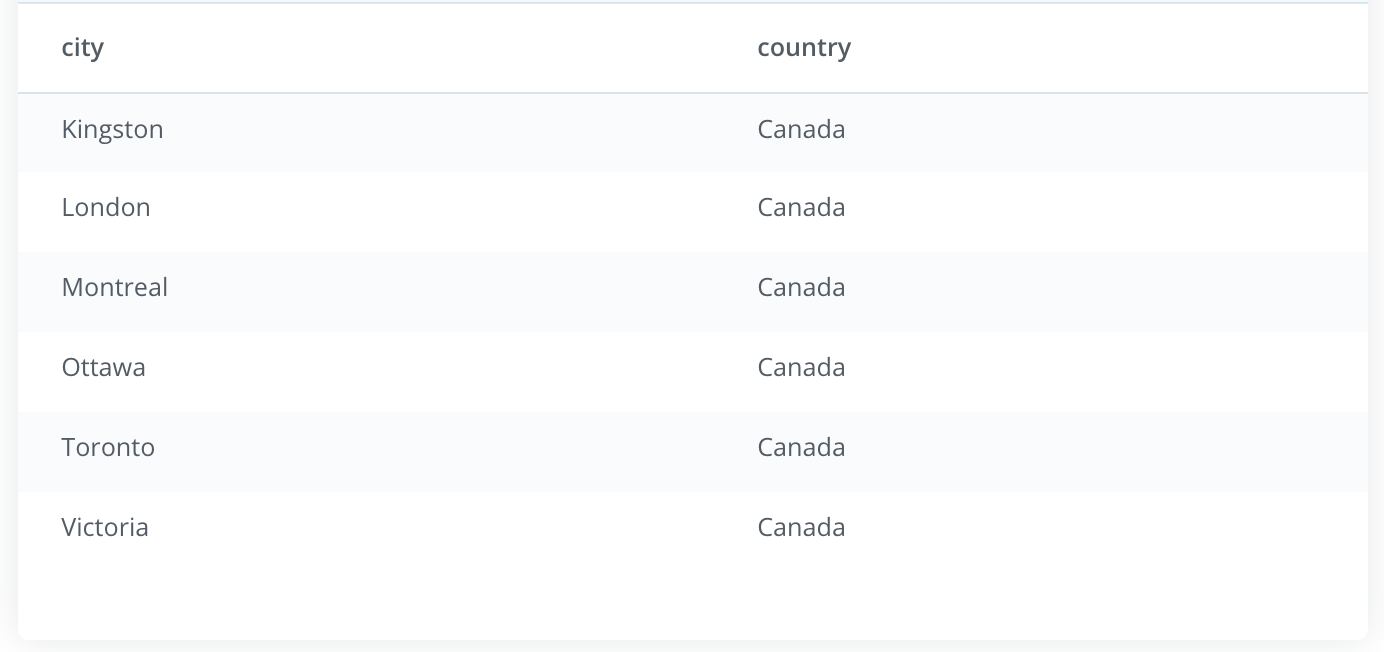
\includegraphics[width=0.85\textwidth]{canada_cities}
    \caption{Cities in Canada.}
  \end{center}
\end{figure}
To extract the data for both the world averages and my city’s averages. We can use these SQL queries:
\begin{center}  
  \begin{tabular}{l}
      SELECT * FROM city\_data WHERE country = 'Canada' AND city = 'London'; \\
      SELECT * FROM global\_data; \\
  \end{tabular}
\end{center}
Here are the results we get from the two queries: 
\begin{figure}[ht]
  \begin{center}
    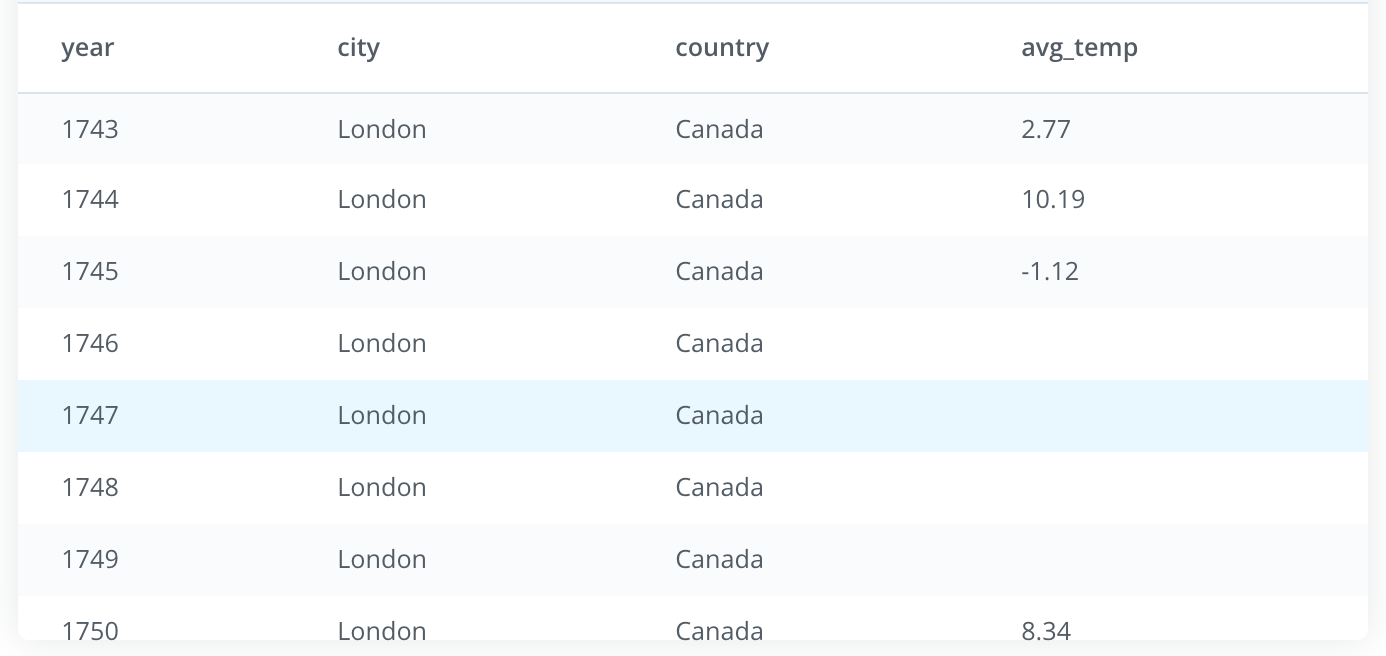
\includegraphics[width=0.85\textwidth]{london_average}
    \caption{London Averages.}
  \end{center}
  \begin{center}
    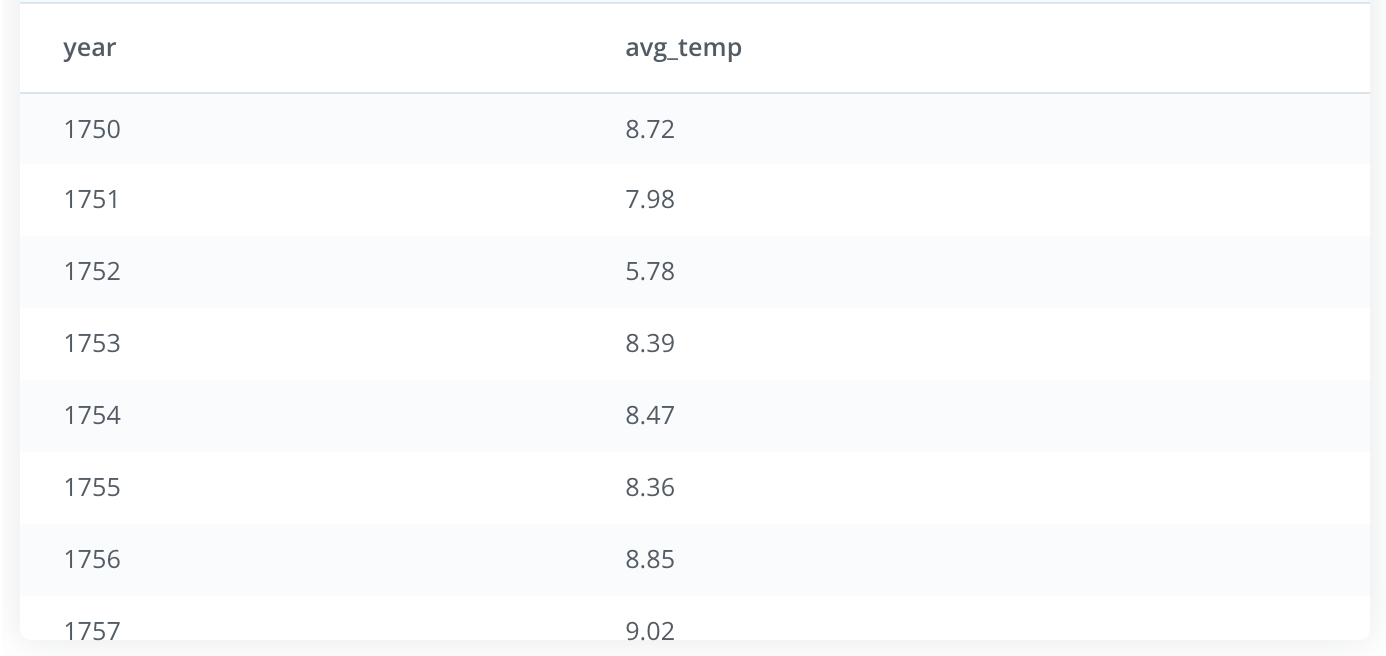
\includegraphics[width=0.85\textwidth]{global_averages}
    \caption{Global Averages.}
  \end{center}
\end{figure}

%----------------------------------------------------------------------------------------
% SECTION 3
%----------------------------------------------------------------------------------------

\section{Open up the CSV}
In Figure 2, some data is missing from 1746 to 1749. Additionally, data from 2014 and 2015 is missing too. To avoid bias, delete missing data is a simple solution. In total, we have 264 rows of data. To smooth out the line, we can use the 12-years moving average. Here is the function for calculating the 12-years MA:
\begin{center} =AVERAGE(D2:D13) \end{center}
Here is part of the yield, after applying the above function cells:
\begin{figure}[ht]
  \begin{center}
    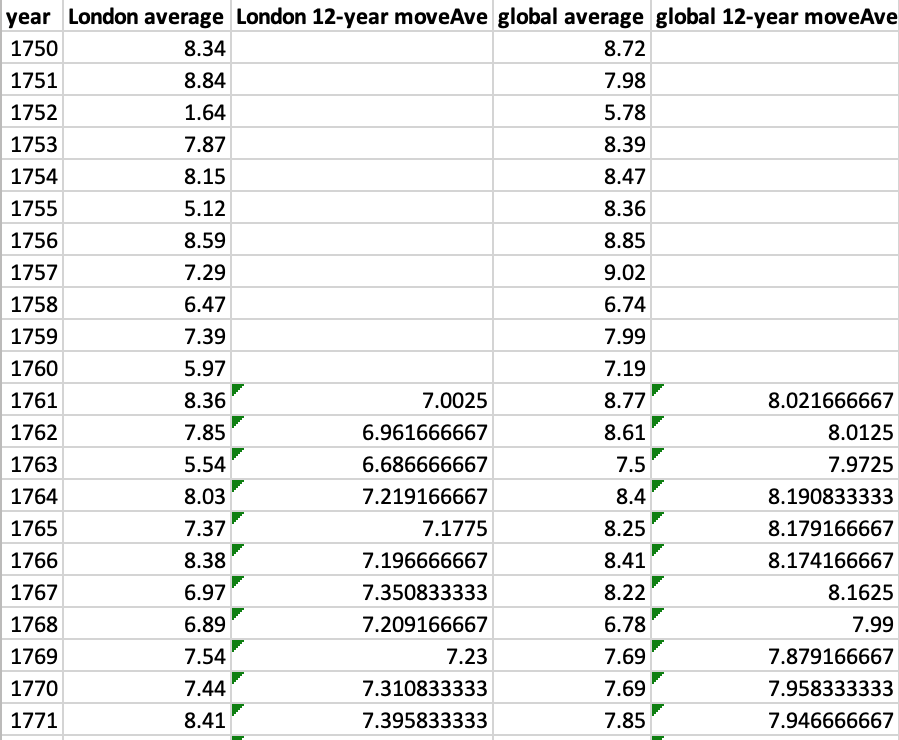
\includegraphics[width=0.75\textwidth]{average_function}
    \caption{Data After Applying 12-Year Moving Average.}
  \end{center}
\end{figure}

%----------------------------------------------------------------------------------------
% SECTION 4
%----------------------------------------------------------------------------------------

\section{Create a line chart}
Here is the line chart:
\begin{figure}[H]
  \begin{center}
    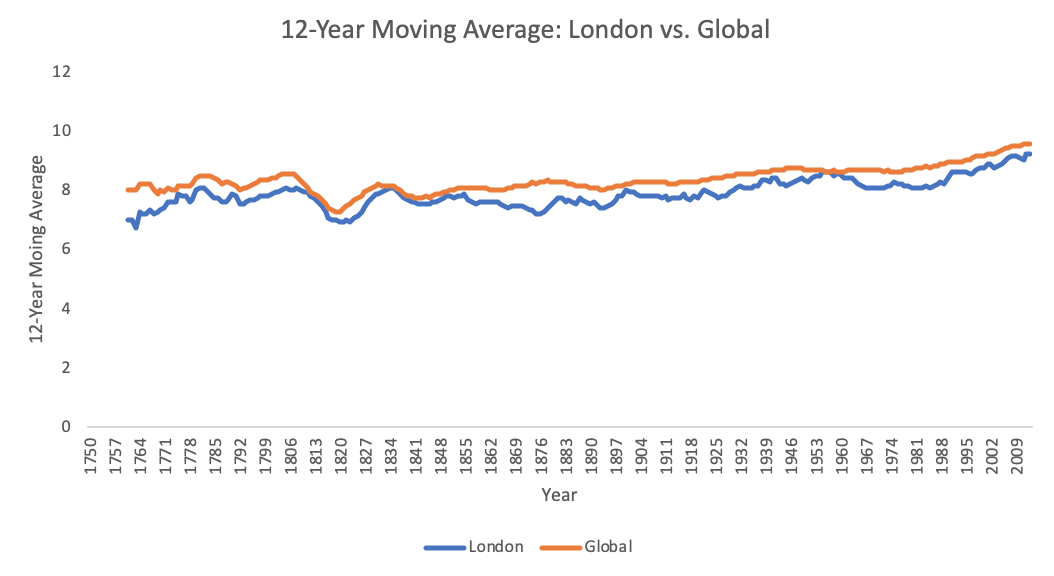
\includegraphics[width=0.95\textwidth]{moving_averages}
    \caption{12-Year Moving Averages}
  \end{center}
\end{figure}


\section{Make observations}
\subsection{Is your city hotter or cooler on average compared to the global average? Has the difference been consistent over time?}
Overall, London is colder on average compared to the global average. However, there are three times that the two standards are nearly touching each other. One happened about 1813, one that happened around 1834, and one that happened roughly in 1955.

\subsection{“How do the changes in your city’s temperatures over time compare to the changes in the global average?”}
Both London and global have similar trends. Before 1841, there is fluctuation occurred in both lines. In around 1806, a severe drop of 2 degrees occurred in both London and global. However, the temperature soon climbed back up around 1828. After 1841 both lines are in an upward trend. The global average is steady, whereas the London average contains various small ups and downs.

\subsection{What does the overall trend look like? Is the world getting hotter or cooler? Has the trend been consistent over the last few hundred years?}
In conclusion, the overall trend is slightly upwards, meaning the world is getting hotter. Over the last few hundred years, the trend is relatively steady.


\end{document}